% Expanded, self-contained explanation of Chapter 6.
% Compile from the repository root:
% latexmk -pdf -outdir=/tmp/full-bst-explained docs/proofs/full-bst-explained.tex
\documentclass[11pt,a4paper]{article}
\usepackage[margin=27mm]{geometry}
\usepackage[T1]{fontenc}
\usepackage[utf8]{inputenc}
\usepackage{lmodern,microtype}
\usepackage{amsmath,amssymb,amsthm}
\usepackage{array,booktabs,longtable,listings,enumitem,needspace,placeins,float}
\usepackage{tikz}
\usetikzlibrary{arrows.meta,positioning}
\usepackage[hidelinks]{hyperref}
\hypersetup{pdftitle={Full BST: a detailed explanation of Chapter 6}}

\newtheoremstyle{readable}{8pt}{6pt}{\normalfont}{}{
  \bfseries}{.}{0.5em}{}
\theoremstyle{readable}
\newtheorem{theorem}{Theorem}[section]
\newtheorem{lemma}[theorem]{Lemma}
\newtheorem{example}[theorem]{Example}
\newcommand{\E}{\mathbb E}
\newcommand{\Prob}{\mathbb P}
\newcommand{\ceil}[1]{\left\lceil #1\right\rceil}
\newcommand{\ind}[1]{\mathbf 1_{\{#1\}}}
\newcommand{\code}[1]{\texttt{#1}}
\setlength{\emergencystretch}{2em}
\setlist{topsep=5pt,itemsep=3pt,parsep=1pt}
\lstset{basicstyle=\small\ttfamily,keywordstyle=\bfseries,
  morekeywords={procedure,while,if,then,else,for,to,do,return,break,end},
  columns=fullflexible,keepspaces=true,showstringspaces=false,
  mathescape=true,frame=tb,framesep=6pt,xleftmargin=1em,captionpos=t}
\tikzset{key/.style={circle,draw,minimum size=7mm,inner sep=1pt},
  subtree/.style={rectangle,draw,fill=black!4,minimum size=6mm,inner sep=3pt},
  gap/.style={rectangle,draw,minimum size=5mm,inner sep=1pt},
  every node/.style={font=\small},
  arr/.style={-{Latex[length=2mm]},thick}}

\title{Full BST\\[0.4em]\large A detailed explanation of Chapter 6}
\author{}
\date{}

\begin{document}
\maketitle
\begin{abstract}
This version explains the algorithm and its proof without relying on the
earlier insertion-only chapter. It assumes familiarity with binary search
trees, logarithms, finite sums, and elementary probability. The probability
inequalities and estimates used in the proof are derived when they are
needed. The purpose is to make each implication explicit; the constants
in the final bounds are sufficient for the proof and are not optimized.
\end{abstract}
\setcounter{section}{5}
\tableofcontents
\clearpage

\section{Full BST: insertion, deletion, and a height bound}
\label{sec:full}

\subsection{The problem, the guarantees, and the assumptions}

A binary search tree, or BST, stores distinct keys in sorted order.
For a node with key $k$, every key in its left subtree is less than $k$,
and every key in its right subtree is greater than $k$. This property
makes search possible, but it does not guarantee that search is fast.
If the tree becomes a chain of $n$ nodes, a search may inspect all $n$ keys.

The algorithm studied here performs a small local repair after each
insertion. It chooses the repair depth at random and makes at most two
rotations. To support deletion, it also periodically removes and
reinserts surviving keys. We call this a \emph{refresh}.

There are two separate quantities to control. The \emph{height} measures
how far a search may have to travel. The number of \emph{pointer changes}
measures how much of the structure is rewritten. A search can read many
pointers while changing none of them, so a constant number of structural
changes does not imply constant operation time.

\paragraph{The guarantees we will prove.}
At any fixed observation time, let $n$ be the number of keys currently
stored. For a suitable fixed sampling probability $p$, we will prove:
\begin{enumerate}
  \item The expected height is $O(\log(n+1))$.
  \item For any chosen constant $\gamma>0$, the probability that the
        height exceeds a suitable constant times $\log n$ is at most
        $n^{-\gamma}$, for $n\ge2$.
  \item An insertion uses at most two rotations. A deletion uses at
        most four rotations and a constant number of other pointer changes.
  \item An operation starting with $n$ keys takes expected
        $O(\log(n+2))$ time under the arithmetic model stated at the end.
\end{enumerate}
The expressions $n+1$ and $n+2$ make the bounds meaningful for small or
empty trees. They do not change the asymptotic growth as $n$ increases.

\paragraph{What is random.}
Fix the entire sequence of public operations in advance, including their
key values. For example, a sequence may insert 20, insert 10, delete 20,
and search for 30. The algorithm then runs this sequence using fresh
independent random trials. Its shapes and heights are random, but the
set of keys after each public operation is fixed by the input sequence.

The theorems do not permit later update keys to be chosen by inspecting
the random shape. Such a choice would make the input itself depend on
the algorithm's randomness. Searches do not change the tree, but the
proof of the update process uses the fixed-sequence assumption.

\paragraph{Why deletion requires extra work.}
Removing a node by ordinary BST deletion does not increase height.
However, this fact compares the new height with the \emph{old height},
not with the logarithm of the \emph{new size}. For example, take a
complete tree and retain only one root-to-leaf path, deleting the other
nodes from the leaves upward. If the original size was $N$, the remaining
chain has about $\log_2 N$ nodes and height of the same order. Its height
is large relative to the logarithm of its new size.

This example explains why an insertion-only bound cannot simply be
carried over to arbitrary deletions. Our refresh schedule continually
establishes a new bound in terms of the current size.

\subsection{The stored information and the basic tree operations}
\label{sec:basics}

Each node stores exactly four fields: its key, left-child pointer,
right-child pointer, and parent pointer. A missing child is null. The
root's parent is null. The tree also stores a root pointer, its size $n$,
and a cursor $c$. The cursor is needed only for the deletion schedule.
Initially $n=0$, the root is null, and $c=-\infty$, a formal value below
all allowed keys.

The cursor stores a \emph{key value}, not a pointer to a node. This
distinction matters because deletion may destroy a node or copy another
key into it. A saved key value can still be compared with the current
keys even after its original node has disappeared.

\paragraph{Depth and height.}
The depth of a node is the number of edges on the path from the root
to that node. The root has depth zero. The height $H$ of a nonempty
tree is the maximum stored-node depth. A tree consisting of one node
therefore has height zero. When useful for discussing updates, we set
the height of the empty tree to $-1$.

\paragraph{Searching for a key.}
At a node with key $x$, compare the query $k$ with $x$. If $k=x$, the
search succeeds. If $k<x$, any occurrence of $k$ must be in the left
subtree, because all keys in the right subtree exceed $x$. Similarly,
if $k>x$, only the right subtree can contain it. Following the selected
child therefore never discards a possible occurrence. Reaching null
proves that the key is absent and identifies its insertion position.

\paragraph{Finding a minimum.}
In a nonempty subtree, follow left children until none remains. Every
left step moves to a smaller key. When no left child exists, all other
keys below the current node lie to its right and are larger, so that
node is the minimum of the original subtree.

\paragraph{Finding the next key after a value.}
The operation $\code{Successor}(c)$ means the least stored key strictly
greater than $c$, even if $c$ itself is absent. Maintain a candidate,
initially null. At a node with key $x>c$, record it and go left: the
right subtree contains only still larger keys and cannot improve on
$x$. At a node with $x\le c$, go right: neither that node nor its left
subtree qualifies. On reaching null, the last candidate is the answer.

\begin{example}[A cursor value that is no longer stored]
Suppose the current set is $\{5,10,25\}$ and the cursor is 20. Its
successor is 25, although 20 is absent. If the cursor is 30, there is
no successor and the schedule must wrap to the minimum, 5. These
answers depend only on the sorted set, not on its tree shape.
\end{example}

\paragraph{One rotation.}
The operation $\code{RotateUp}(x)$ promotes a nonroot node $x$ above
its parent. Figure~\ref{fig:rotation} shows the case where $x$ is a
right child. The letters $A,B,C$ denote entire subtrees, any of which
may be empty. Every key in them satisfies the same inequalities as
their positions suggest.

\begin{figure}[htbp]
\centering
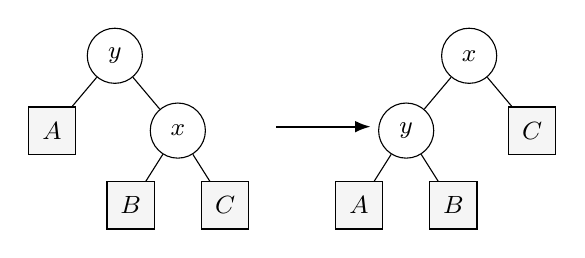
\begin{tikzpicture}[x=1cm,y=1cm]
  \node[key] (y) at (0,0) {$y$};
  \node[subtree] (A) at (-.8,-.95) {$A$};
  \node[key] (x) at (.8,-.95) {$x$};
  \node[subtree] (B) at (.2,-1.9) {$B$};
  \node[subtree] (C) at (1.4,-1.9) {$C$};
  \draw (A)--(y)--(x)--(B) (x)--(C);
  \draw[arr] (2.05,-.9)--(3.25,-.9);
  \node[key] (xx) at (4.5,0) {$x$};
  \node[key] (yy) at (3.7,-.95) {$y$};
  \node[subtree] (AA) at (3.1,-1.9) {$A$};
  \node[subtree] (BB) at (4.3,-1.9) {$B$};
  \node[subtree] (CC) at (5.3,-.95) {$C$};
  \draw (AA)--(yy)--(xx)--(CC) (yy)--(BB);
\end{tikzpicture}
\caption{Promoting a right child. The middle subtree $B$ changes
parent, but remains between $y$ and $x$ in sorted order.}
\label{fig:rotation}
\end{figure}

Before the rotation, the inorder order is $A,y,B,x,C$. Afterward it is
still $A,y,B,x,C$. In particular, every key in $B$ lies between $y$
and $x$, so moving $B$ from the left of $x$ to the right of $y$ preserves
the BST property. The left-child case reverses left and right.

A rotation changes only the links between these nodes, the middle
subtree, and the old parent of $y$. If $y$ was the root, update the root
pointer. Repair the parent pointer of each subtree whose parent changes.
This is a constant number of pointer writes, independent of the sizes
of $A,B,C$; their internal links are not visited or changed.

\paragraph{Removing a node with at most one child.}
To splice out such a node $u$, let $b$ be its child, or null if there
is none. Replace the pointer from $u$'s parent to $u$ by $b$, and set
$b$'s parent to $u$'s old parent when $b$ is nonnull. If $u$ was the
root, set the root to $b$. Finally clear all three links of $u$.
Every node in the promoted child's subtree moves up one level; all
other stored nodes keep their depths. This operation cannot increase
height and also takes a constant number of pointer writes.

\FloatBarrier
\subsection{Insertion and the distribution of the target}
\label{sec:insertion}

Fix a number $p$ with
\[
  \frac{\sqrt5-1}{2}<p<1.
\]
A Bernoulli$(p)$ trial is a random experiment that succeeds with
probability $p$ and fails with probability $1-p$. All trials are fresh
and independent: knowing previous outcomes does not change the
probabilities of the next trial. Section~\ref{sec:weight-estimate}
will derive the reason for the lower bound on $p$.

\subsubsection*{Attaching the leaf and sampling a depth}
Use ordinary BST insertion to attach the new key as a leaf. Let $v$
be the new node, $d$ its depth immediately after attachment, and $n$
the size including this new node. Define
\[
  \ell_n=\ceil{\log_{1/p}n}.
\]
Because $0<p<1$, the base $1/p$ is greater than one. Thus $\ell_n$
grows logarithmically with $n$.

The target starts at $t=\ell_n$. While $t>0$, perform a trial. A success
decreases $t$ by one; a failure ends sampling. Reaching zero also ends
sampling. The random variable denoting the final target is $T_n$ when
the insertion ends at size $n$. Different insertions at the same size
use different independent samples with this same distribution.

The target is an \emph{absolute depth measured from the root}. It is
not the number of edges to move upward from the new leaf. For example,
if the leaf is at depth 20 and the target is 3, repair happens near
depth 3; the leaf is not rotated all the way to depth 3.

\begin{lemma}[The target distribution]
\label{lem:target}
For an insertion ending at size $n\ge1$,
\begin{align}
  \Prob(T_n=0)&=p^{\ell_n}, \label{eq:target-zero}\\
  \Prob(T_n=t)&=(1-p)p^{\ell_n-t}
        &&(1\le t\le\ell_n), \label{eq:target-mass}\\
  \Prob(T_n\le t)&=p^{\ell_n-t}
        &&(0\le t\le\ell_n). \label{eq:target-cdf}
\end{align}
These formulas hold even after conditioning on all the preceding random
choices. Also $p^{\ell_n}\le1/n$.
\end{lemma}

\begin{proof}
To reach a positive target $t$ and stop there, the first $\ell_n-t$
trials must succeed and the next must fail. Independence makes the
probability the product $p^{\ell_n-t}(1-p)$.

To reach zero, exactly $\ell_n$ initial successes are required. No
failure is needed afterward, because the loop stops at zero. This gives
$p^{\ell_n}$. When $\ell_n=0$, this probability is $p^0=1$ and the
algorithm performs no trials.

The event $T_n\le t$ says that sampling reaches depth $t$ or goes
farther toward the root. It requires the first $\ell_n-t$ trials to
succeed, with no restriction on later trials. Its probability is
therefore $p^{\ell_n-t}$.

These probabilities add to one. For $\ell_n>0$, their positive-target
sum is
\[
 (1-p)\sum_{j=0}^{\ell_n-1}p^j
   =(1-p)\frac{1-p^{\ell_n}}{1-p}=1-p^{\ell_n}.
\]
Adding the mass at zero gives one; the case $\ell_n=0$ was already
handled. Finally, the definition of the ceiling gives
$(1/p)^{\ell_n}\ge n$. Taking reciprocals, which reverses an inequality
between positive numbers, gives $p^{\ell_n}\le1/n$.

The trials used now are independent of the previous history. Fixing
that history therefore does not change any of the probabilities above.
\end{proof}

\begin{example}[The complete target distribution for three keys]
Take $p=2/3$ and $n=3$. Since $(3/2)^2=9/4<3$ and
$(3/2)^3=27/8\ge3$, the ceiling is $\ell_3=3$. Write S for success
and F for failure. The possible stopping outcomes are:
\begin{center}
\begin{tabular}{cccc}
\toprule
Target & Outcomes & Probability calculation & Probability \\
\midrule
3 & F & $1-p$ & $1/3$ \\
2 & SF & $p(1-p)$ & $2/9$ \\
1 & SSF & $p^2(1-p)$ & $4/27$ \\
0 & SSS & $p^3$ & $8/27$ \\
\bottomrule
\end{tabular}
\end{center}
The four probabilities sum to $(9+6+4+8)/27=1$. The zero-target
probability is $8/27\le1/3$, as the lemma predicts.
\end{example}

\subsubsection*{The repair rule}
The target determines which part of the insertion path is repaired.
\begin{enumerate}
  \item If $d\le t$, the leaf is already at or above the target, and
        there is no repair.
  \item If $d=t+1$, the leaf is exactly one level below it. Rotate
        the leaf up once.
  \item If $d\ge t+2$, let $g,y,x$ be the nodes on the insertion
        path at depths $t,t+1,t+2$. If both edges have the same
        direction, rotate $y$ up once. If the directions differ,
        rotate $x$ up twice.
\end{enumerate}
The third case uses a \emph{straight} path for left--left or right--right,
and a \emph{bent} path for left--right or right--left. We use $y$ for
the middle node so that $p$ continues to denote a probability.

\Needspace{24\baselineskip}
\noindent\begin{minipage}{\linewidth}
\begin{lstlisting}[caption={Repair; the probability $p$ is fixed globally.}]
Repair($v,n,d$):
    $t \gets \lceil\log_{1/p}n\rceil$
    while $t>0$:
        if Bernoulli($p$) = 0: break
        $t \gets t-1$
    if $d\le t$: return
    if $d=t+1$:
        RotateUp($v$)
        return

    $x \gets v$
    for $i=1$ to $d-t-2$:
        $x \gets x$.parent
    $y \gets x$.parent
    $g \gets y$.parent
    if $(x=y.\mathrm{left})\Longleftrightarrow(y=g.\mathrm{left})$:
        RotateUp($y$)
    else:
        RotateUp($x$)
        RotateUp($x$)
\end{lstlisting}
\end{minipage}

After $k$ parent steps from a node at depth $d$, its ancestor has depth
$d-k$. To reach depth $t+2$, solve $d-k=t+2$, giving $k=d-t-2$.
This explains the loop bound. The third case guarantees that this
number is nonnegative. If it is zero, $x$ is the new leaf itself.
Since $t\ge0$, a node at depth $t+2$ has both a parent and a grandparent,
so $y$ and $g$ exist.

Every case preserves BST order, because attaching the leaf uses the
search position and each subsequent rotation preserves inorder order.
There are zero, one, or two rotations. For the first insertion, $n=1$,
$\ell_1=0$, and $d=0$, so the new root is unchanged.

\begin{example}[The promoted node need not be the new leaf]
Suppose a new leaf is attached at depth 8 and the target is 2. The
parent loop takes $8-2-2=4$ steps to reach $x$ at depth 4. Repair
involves depths 2, 3, and 4, although the inserted leaf is still
farther down the path. On a straight path the leaf moves up only one
level, from depth 8 to depth 7. This is why the analysis must track the
effects on subtrees, rather than assuming that the new key reaches
the sampled target.
\end{example}

\subsubsection*{Public insertion and raw insertion}
A public insertion does nothing if its key is already stored. Its search
can detect this before making any change. Otherwise it attaches a new
node, increments the size, and calls \code{Repair} with the depth
computed by the search.

We also use $\code{RawInsert}(v)$ during a refresh. Its precondition is
that $v$ is a detached node and its key is absent. It performs the same
leaf insertion, size increment, and repair, reusing $v$ instead of
allocating a new node. Neither public insertion nor raw insertion changes
the cursor. The distinction is about the caller's guarantees and memory
reuse; both successful insertions have the same random repair rule.

\Needspace{13\baselineskip}
\subsection{Deletion, refreshes, and moving the minimum}
\label{sec:deletion}

\subsubsection*{Raw removal: which node is actually detached}
To remove a key at node $z$, use one of two cases.
\begin{itemize}
  \item If $z$ has no right child, splice out $z$, promoting its left
        child when present.
  \item If $z$ has a right child, find $u=\code{Minimum}(z.\mathrm{right})$.
        Copy $u$'s key into $z$ and splice out $u$, promoting $u$'s
        right child when present.
\end{itemize}
In the second case, $u$ has no left child: a left child would be a
smaller key in the same subtree and contradict the choice of $u$ as
its minimum. Thus both cases reduce to a splice with at most one child.

The copied key is the successor of the removed key. It exceeds every
key in $z$'s left subtree and is smaller than every other key in $z$'s
right subtree. It also belonged to $z$'s original subtree, so it satisfies
the ordering restrictions imposed by $z$'s ancestors. Replacing the key
and then splicing out its old occurrence therefore preserves BST order.

\Needspace{16\baselineskip}
\noindent\begin{minipage}{\linewidth}
\begin{lstlisting}[caption={Raw removal returns a detached node for reuse.}]
RawRemove($z$):
    if $z$.right is null:
        $u \gets z$
        splice out $u$, promoting $u$.left
    else:
        $u \gets$ Minimum($z$.right)
        $z$.key $\gets u$.key
        splice out $u$, promoting $u$.right
    decrement $n$
    return $u$
\end{lstlisting}
\end{minipage}

In particular, we use the successor case even when $z$ has only a
right child. Promoting that whole child would also preserve search
order, but the proof below uses the stated successor rule to carry a
gap bound from left to right. The algorithm must use the rule being
analyzed.

The returned node is a physical memory object. It may contain the
successor's key rather than the key requested for removal. This matters
when the node is reused during a refresh.

\subsubsection*{A refresh removes and reinserts the same key}
The next refreshed key is the least key greater than the cursor $c$.
If no such key exists, choose the current minimum and move it directly
to the root before refreshing it. Afterward, save the refreshed key's
value as the new cursor.

\Needspace{29\baselineskip}
\noindent\begin{minipage}{\linewidth}
\begin{lstlisting}[caption={A public deletion and one step of its refresh schedule.}]
Delete($k$):
    $z \gets$ Search($k$)
    if $z$ is null: return
    free the node returned by RawRemove($z$)
    if $n=0$:
        $c \gets -\infty$
        return
    RefreshNext()
    RefreshNext()

RefreshNext():                 // precondition: $n>0$
    $z \gets$ Successor($c$)
    if $z$ is null:
        $z \gets$ Minimum(root)
        MoveMinimumToRoot($z$)
    $k \gets z$.key
    $u \gets$ RawRemove($z$)
    $u$.key $\gets k$
    RawInsert($u$)
    $c \gets k$
\end{lstlisting}
\end{minipage}

Let $S$ be the set just before a refresh, and let $k$ be the chosen key.
Raw removal leaves $S\setminus\{k\}$. Assigning the saved value $k$
to the detached node and reinserting it gives
$(S\setminus\{k\})\cup\{k\}=S$. Thus a refresh changes shape but
not the set. Each raw insertion uses fresh random trials, including
when it reinserts a previously stored key.

Raw operations leave the cursor alone. If the only remaining key is
refreshed, raw removal temporarily empties the tree, but the cursor is
not reset. Reinsertion restores the singleton, and the refresh then
assigns its key to the cursor. Both refreshes in a deletion may visit
this same singleton. Only a public deletion that leaves no keys resets
the cursor to $-\infty$.

\subsubsection*{The direct minimum-to-root move}
Let $m$ be the minimum. It has no left child. If it is not the root,
it must be a left child: being a right child would make its parent a
smaller stored key. Detach $m$ by putting its right child in its old
position. All keys in the remaining tree are greater than $m$, so the
entire remaining tree can be attached as $m$'s right subtree.

\Needspace{16\baselineskip}
\noindent\begin{minipage}{\linewidth}
\begin{lstlisting}[caption={Moving the minimum without a chain of rotations.}]
MoveMinimumToRoot($m$):
    if $m$ = root: return
    $parent \gets m$.parent
    $parent$.left $\gets m$.right
    if $parent$.left is not null:
        $parent$.left.parent $\gets parent$
    $m$.right $\gets$ root
    root.parent $\gets m$
    $m$.parent $\gets$ null
    root $\gets m$
\end{lstlisting}
\end{minipage}

The move retains the same nodes and keys. Its pointer writes are
constant in number even when the minimum is very deep. Finding the
minimum still takes a walk down the tree. If the minimum has depth
$d$, promoting it by ordinary rotations would require at least $d$
rotations, because one rotation reduces its depth by at most one.
The direct move is therefore an additional primitive, not a rotation
sequence counted as one rotation.

\begin{example}[One deletion, including both refreshes]
Begin with root 20, left child 10, right child 30, and $c=-\infty$.
Suppose both reinsertions sample a target of at least one.
\begin{enumerate}
  \item Removing 20 copies successor key 30 into the root and detaches
        the old node holding 30. The surviving root is 30 with left
        child 10, and the size is two.
  \item The least key above $-\infty$ is 10. Removing and reinserting
        10 attaches it again at depth one. Because $d=1\le t$, no
        rotation occurs. Set $c=10$.
  \item The next key is 30. It has no right child, so removing it
        promotes 10 to the root. Reinserting 30 attaches it as the
        right child of 10 at depth one. Again there is no repair.
        Set $c=30$.
\end{enumerate}
The final set is $\{10,30\}$, exactly the original set minus 20.
The refreshes changed its shape while preserving this set.

Now insert 5 and 25, choosing outcomes that require no repair, and
delete 30. Its left child 25 takes its place. The surviving set is
$\{5,10,25\}$, but the cursor still holds 30. The first refresh finds
no larger key, moves 5 to the root, and refreshes 5. The second visits
10. In particular, the identity of the second refreshed key does not
depend on the first refresh's random rotations.
\end{example}

\subsection{The proof's objects: gaps, weights, and expectation}
\label{sec:probability}

\subsubsection*{Why follow gaps instead of node identities}
Write the current keys in increasing order as $k_1<\cdots<k_n$.
The $n+1$ gaps are the positions before $k_1$, between each consecutive
pair, and after $k_n$. We denote them by $G_0,\ldots,G_n$:
\[
  G_0,\ k_1,\ G_1,\ k_2,\ \ldots,\ k_n,\ G_n.
\]
A gap describes a position in sorted order, even if an application's
integer key domain has no available integer between two adjacent keys.
For reasoning about comparisons, one may imagine the keys on a number
line and place a query between them.

An unsuccessful search in a gap ends at a particular null child pointer.
Regard this pointer as an \emph{external leaf} one level below its parent.
For example, in a tree with root 20 and children 10 and 30, all four
gaps have depth two. Queries below 10 reach the left null pointer of 10;
queries between 10 and 20 reach its right null pointer; the other two
gaps are below 30.

These external leaves require no storage. A nonempty tree has $2n$
child-pointer fields, of which $n-1$ are nonnull edges between stored
nodes, one for each nonroot node. Thus $2n-(n-1)=n+1$ child pointers
are null, agreeing with the
number of gaps.

If a gap has depth $D$, searching for a query in it makes $D$ key
comparisons: the path visits stored nodes at depths $0,\ldots,D-1$
and then reaches null. The deepest gap has depth $H+1$. No gap can be
deeper, because its parent has depth at most $H$. A stored node at
maximum depth has no child, so one of its null pointers attains $H+1$.

Insertion splits one gap into two. Removal merges the two gaps adjacent
to the removed key. This description follows the key order even when
the implementation copies a successor's key to another node. It avoids
having to identify a logical key with one permanent memory address.

\subsubsection*{A weight that detects unusually large depths}
For the moment, let $a>1$ be a constant. Give a gap of depth $D$ weight
$W=a^D$. Increasing depth by one multiplies the weight by $a$;
decreasing depth by one multiplies it by $a^{-1}=1/a$.

The exponential function puts a large penalty on a very deep gap.
This is useful because we want to bound the \emph{maximum} depth.
Knowing only a small expected depth for each individual gap would not,
by itself, give the logarithmic bound for their maximum that we need.

\paragraph{Markov's inequality, with its proof.}
For any nonnegative random variable $X$ and any $b>0$,
\[
  X\ge b\,\ind{X\ge b}.
\]
Here the indicator is one when its condition is true and zero otherwise.
On the event $X\ge b$ the inequality says $X\ge b$; outside that
event it says $X\ge0$. Taking expectations gives
\[
  \E[X]\ge b\Prob(X\ge b),
  \qquad\text{so}\qquad
  \Prob(X\ge b)\le\frac{\E[X]}b.
\]
Set $X=a^D$ and $b=a^h$. Since $a>1$, the events $a^D\ge a^h$
and $D\ge h$ are the same. Hence
\begin{equation}
  \Prob(D\ge h)\le\frac{\E[a^D]}{a^h}.
  \label{eq:markov}
\end{equation}

It is enough for the numerator to be polynomial in the size. For example,
if $\E[a^D]\le C(n+1)^b$ and
$h=\log_a C+(b+\gamma)\log_a(n+1)$, substitution gives
\[
  \frac{C(n+1)^b}{a^h}=(n+1)^{-\gamma}.
\]
The numerator need not be constant. A logarithmic threshold makes the
exponential denominator dominate any fixed polynomial numerator.

\paragraph{The union bound, with its proof.}
For events $E_1,\ldots,E_m$, the indicator that at least one occurs is
at most the sum of their indicators. Taking expectations gives
\[
  \Prob(E_1\cup\cdots\cup E_m)
    \le\sum_{i=1}^m\Prob(E_i).
\]
No independence is used. We will apply this to the events that particular
gaps are too deep. Their depths can be strongly dependent, because they
belong to the same random tree.

\subsubsection*{Conditioning first and averaging afterward}
A local insertion estimate is easiest to prove with the current tree
held fixed. Its old gap weights are then ordinary numbers, and the
only randomness is the new target. Suppose this argument proves
\[
  \E[W'\mid\text{current tree}]
     \le\lambda W+B
\]
for constants $\lambda,B$ determined by the size. The vertical bar
means that we temporarily regard the current tree as known.

To return to the actual random tree, average this inequality over its
possible shapes. Writing $\tau$ for a possible tree gives
\begin{align*}
  \E[W']
  &=\sum_\tau\Prob(\text{tree}=\tau)
       \E[W'\mid\text{tree}=\tau]\\
  &\le\sum_\tau\Prob(\text{tree}=\tau)
       \bigl(\lambda W(\tau)+B\bigr)\\
  &=\lambda\E[W]+B.
\end{align*}
The first equality is the law of total expectation; here it is simply
a weighted average over the possible current trees. The old depth and
new depth are not assumed independent. Freshness of the new trials is
what lets us use the same target distribution after fixing the old tree.

\paragraph{The route through the rest of the proof.}
We first determine exactly how one repair changes gap depths. We then
choose $a$ so that the main increases and decreases cancel in expected
weight. Raw removal will transfer the bound from the left gap of a key
to the gap produced by its removal. An increasing sweep will carry a
bound across every key. Finally, we will bound the accumulated growth
within a sweep and convert the resulting weight bound into a height bound.

\subsection{Exactly how one repair changes gap depths}
\label{sec:local-effects}

There are two different situations: insertion into another gap, and
insertion into the gap being followed. They must be treated separately
because only the second situation splits that gap.

\subsubsection*{The two rotation patterns, including their subtrees}
Suppose the repair uses $g,y,x$ at depths $t,t+1,t+2$. The following
diagrams include all subtrees hanging from these three nodes. A letter
such as $A$ denotes the same unchanged subtree before and after repair.
If it is empty, its attachment position is an external gap. If it is
nonempty, every node and gap inside it changes depth by the change in
its attachment depth.

\begin{figure}[H]
\centering
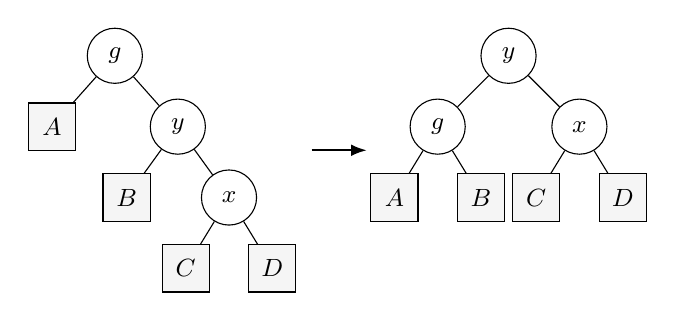
\begin{tikzpicture}
  \node[key] (g) at (0,0) {$g$};
  \node[subtree] (A) at (-.8,-.9) {$A$};
  \node[key] (y) at (.8,-.9) {$y$};
  \node[subtree] (B) at (.15,-1.8) {$B$};
  \node[key] (x) at (1.45,-1.8) {$x$};
  \node[subtree] (C) at (.9,-2.7) {$C$};
  \node[subtree] (D) at (2,-2.7) {$D$};
  \draw (A)--(g)--(y)--(B) (y)--(x)--(C) (x)--(D);
  \draw[arr] (2.5,-1.2)--(3.2,-1.2);
  \node[key] (yy) at (5,0) {$y$};
  \node[key] (gg) at (4.1,-.9) {$g$};
  \node[key] (xx) at (5.9,-.9) {$x$};
  \node[subtree] (AA) at (3.55,-1.8) {$A$};
  \node[subtree] (BB) at (4.65,-1.8) {$B$};
  \node[subtree] (CC) at (5.35,-1.8) {$C$};
  \node[subtree] (DD) at (6.45,-1.8) {$D$};
  \draw (AA)--(gg)--(yy)--(xx)--(CC) (gg)--(BB) (xx)--(DD);
\end{tikzpicture}

\smallskip
\begin{tabular}{ccccc}
\toprule
Subtree & $A$ & $B$ & $C$ & $D$ \\
\midrule
Old attachment depth & $t+1$ & $t+2$ & $t+3$ & $t+3$ \\
New attachment depth & $t+2$ & $t+2$ & $t+2$ & $t+2$ \\
Change & $+1$ & $0$ & $-1$ & $-1$ \\
\bottomrule
\end{tabular}
\caption{Straight right--right repair: rotate $y$ above $g$ once.
The top of each drawing is at depth $t$.}
\label{fig:straight}
\end{figure}

For the straight case in Figure~\ref{fig:straight}, $y$ moves to
depth $t$ and $g$ moves down to depth $t+1$. Subtree $A$ stays attached
to $g$, so it moves down with it. Subtree $B$ changes from the left
of $y$ to the right of $g$; its old and new attachment depths are both
$t+2$. Node $x$ stays below $y$ and therefore moves up one level.
Both of its original child subtrees, $C$ and $D$, move up with it.
The left--left case is obtained by exchanging left and right everywhere;
none of these depth differences changes.

\begin{figure}[H]
\centering
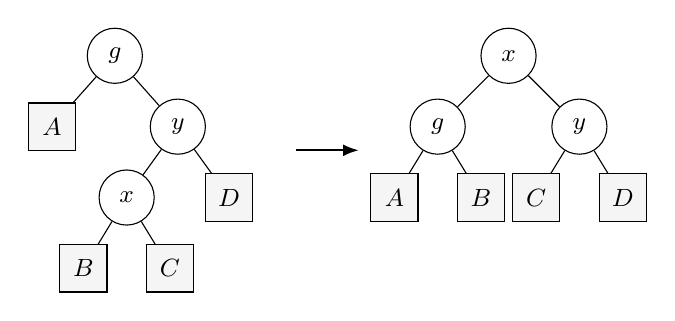
\begin{tikzpicture}
  \node[key] (g) at (0,0) {$g$};
  \node[subtree] (A) at (-.8,-.9) {$A$};
  \node[key] (y) at (.8,-.9) {$y$};
  \node[key] (x) at (.15,-1.8) {$x$};
  \node[subtree] (D) at (1.45,-1.8) {$D$};
  \node[subtree] (B) at (-.4,-2.7) {$B$};
  \node[subtree] (C) at (.7,-2.7) {$C$};
  \draw (A)--(g)--(y)--(x)--(B) (x)--(C) (y)--(D);
  \draw[arr] (2.3,-1.2)--(3.1,-1.2);
  \node[key] (xx) at (5,0) {$x$};
  \node[key] (gg) at (4.1,-.9) {$g$};
  \node[key] (yy) at (5.9,-.9) {$y$};
  \node[subtree] (AA) at (3.55,-1.8) {$A$};
  \node[subtree] (BB) at (4.65,-1.8) {$B$};
  \node[subtree] (CC) at (5.35,-1.8) {$C$};
  \node[subtree] (DD) at (6.45,-1.8) {$D$};
  \draw (AA)--(gg)--(xx)--(yy)--(CC) (gg)--(BB) (yy)--(DD);
\end{tikzpicture}

\smallskip
\begin{tabular}{ccccc}
\toprule
Subtree & $A$ & $B$ & $C$ & $D$ \\
\midrule
Old attachment depth & $t+1$ & $t+3$ & $t+3$ & $t+2$ \\
New attachment depth & $t+2$ & $t+2$ & $t+2$ & $t+2$ \\
Change & $+1$ & $-1$ & $-1$ & $0$ \\
\bottomrule
\end{tabular}
\caption{Bent right--left repair: rotate $x$ above $y$, then above
$g$. The top of each drawing is at depth $t$.}
\label{fig:bent}
\end{figure}

For the bent case in Figure~\ref{fig:bent}, the first rotation makes
$x$ the right child of $g$ and makes $y$ the right child of $x$.
Subtree $C$ becomes the left subtree of $y$. The second rotation
promotes $x$ above $g$ and makes $B$ the right subtree of $g$.
This gives the final drawing. Reading off depths gives the table:
$A$ moves down one level, $D$ keeps its depth, and $B,C$ each move
up one level. Although $x$ itself moves up \emph{two} levels, its two
original child subtrees move up only \emph{one}. The left--right case
has exactly the same depth changes after exchanging left and right.

\FloatBarrier
\subsubsection*{Insertion into a different gap}
Fix a query in a gap other than the insertion gap. Let $D$ be its
external depth before insertion and $D'$ its depth afterward. The two
search paths agree from the root until a stored node at some depth $s$;
at this node they take different children. We call $s$ the divergence
depth. Attaching the new leaf does not affect the query's gap, so only
the repair can change its depth.

For the three-node repair, the diagrams give all possibilities:
\begin{enumerate}
  \item If $t=s$, the paths diverge at $g$. The query is in the
        subtree opposite $y$, labeled $A$ in either diagram. Its
        depth increases by one.
  \item If $t=s-1$, the paths diverge at $y$. The query is in the
        subtree opposite $x$: $B$ in the straight diagram and $D$
        in the bent diagram. Its depth stays unchanged.
  \item If $t\le s-2$, the paths agree through $x$, because
        $s\ge t+2$. The query's external leaf lies in an original
        child subtree of $x$. Either diagram moves that subtree up
        one level, so the query depth decreases by one.
  \item If $t>s$, the paths diverge before reaching the repair
        subtree. No pointer on the remaining query path changes,
        so its depth stays unchanged.
\end{enumerate}

The boundary cases fit the same rule. If repair rotates only the new
leaf, $d=t+1$. A different-gap query can diverge at its parent, of
depth $t$, or earlier. Divergence at the parent places it in the
opposite subtree, which moves down one; earlier divergence leaves it
unaffected. If no rotation occurs, $t\ge d$. Different paths must
diverge at some $s\le d-1$, so $t>s$ and the query is unaffected.
We have therefore proved the exact rule
\begin{equation}
  D'-D=
  \begin{cases}
    +1,&t=s,\\
    0,&t=s-1,\\
    -1,&0\le t\le s-2,\\
    0,&t>s.
  \end{cases}
  \label{eq:depth-change}
\end{equation}
Conditions requiring a negative target simply cannot occur.

\subsubsection*{Insertion into the gap being followed}
Now the insertion replaces an external leaf of depth $D$ by a stored
leaf at that depth and two new external leaves at depth $D+1$.
Examine the same three repair cases:
\begin{itemize}
  \item If $t\ge D$, no repair occurs and both new gaps remain at
        depth $D+1$.
  \item If $t=D-1$, the new node rotates above its parent. Its outer
        null pointer moves up one level to depth $D$. Its inner null
        pointer becomes a child pointer of the former parent and stays
        at depth $D+1$. Thus the two depths are $D$ and $D+1$.
  \item If $t\le D-2$, the repair uses three nodes. If the new leaf
        is strictly below $x$, both new gaps lie in an original child
        subtree of $x$ and move up one level. If $x$ is the new leaf
        itself, a straight repair moves it and both null children up
        one level. In a bent repair, its two null children become the
        inner child pointers of the old ancestors $g,y$, both at
        depth $t+2=D$. In all these cases both new gaps finish at $D$.
\end{itemize}
In particular, neither new gap finishes deeper than $D+1$. If
$D\ge\ell_n+2$, then every possible target satisfies
$t\le\ell_n\le D-2$, so both new gaps finish at depth $D$ for
\emph{every} random outcome.

\subsection{Choosing the weight and proving the insertion estimate}
\label{sec:weight-estimate}

We now choose the base $a$ rather than assuming it. Fix the current
tree and consider a different-gap insertion whose divergence depth
satisfies $2\le s\le\ell_n$. Write $P_+$ for the probability that
the query depth increases by one, and $P_-$ for the probability that
it decreases by one. Equation~\eqref{eq:depth-change} and
Lemma~\ref{lem:target} give
\begin{align*}
  P_+&=\Prob(T_n=s)=(1-p)p^{\ell_n-s},\\
  P_-&=\Prob(T_n\le s-2)=p^{\ell_n-(s-2)}
       =p^{\ell_n-s+2}.
\end{align*}
The probabilities share the positive factor $p^{\ell_n-s}$, so
\[
  \frac{P_-}{P_+}=\frac{p^2}{1-p}.
\]
This ratio does not depend on the current size, depth, or shape.

\subsubsection*{The cancellation, term by term}
The multiplier of the old weight is $a$ on a one-level increase,
$a^{-1}$ on a one-level decrease, and 1 otherwise. Therefore
\begin{align*}
  \E[a^{D'-D}\mid\text{current tree}]
   &=P_+a+P_-a^{-1}+(1-P_+-P_-)\\
   &=1+P_+(a-1)+P_-(a^{-1}-1)\\
   &=1+(a-1)\left(P_+-\frac{P_-}{a}\right).
\end{align*}
In the last line we used $a^{-1}-1=-(a-1)/a$. Choosing
\begin{equation}
  a=\frac{p^2}{1-p}
  \label{eq:a}
\end{equation}
makes $P_-=aP_+$, so the expression in parentheses is zero. The
conditional expected multiplier is exactly one. Since the old depth
$D$ is fixed while conditioning on the tree,
\[
  \E[a^{D'}\mid\text{current tree}]
     =a^D\E[a^{D'-D}\mid\text{current tree}]=a^D.
\]
This equality is about expected \emph{weight}. It does not say that
the depth stays unchanged on each execution, or that the expected
depth change itself is zero.

For example, when $p=2/3$, the selected base is $a=4/3$.
Increasing depth adds $1/3$ of the old weight. Decreasing depth
subtracts $1/4$ of it. A decrease is $4/3$ times as probable as an
increase, so the two expected contributions are
\[
  P_+\frac13
   \quad\text{and}\quad
  -\frac43P_+\frac14=-P_+\frac13.
\]
Their sum is zero.

\subsubsection*{Why the restriction on the sampling probability appears}
The tail argument needs $a>1$, so that larger depths have larger
weights. With the choice in \eqref{eq:a}, this condition becomes
\begin{align*}
  \frac{p^2}{1-p}>1
  &\quad\Longleftrightarrow\quad p^2>1-p\\
  &\quad\Longleftrightarrow\quad p^2+p-1>0.
\end{align*}
The two roots of $p^2+p-1$ are $(-1-\sqrt5)/2$ and
$(-1+\sqrt5)/2$. The first is negative. The quadratic opens upward,
so for $0<p<1$ it is positive exactly when
$p>(\sqrt5-1)/2$. This derives the assumption used in the algorithm.
It is a sufficient condition for this proof; the calculation alone
does not settle the behavior for smaller probabilities.

\subsubsection*{The exceptional divergence depths}
The cancellation handled $2\le s\le\ell_n$. The other depths
must be checked separately.
\begin{itemize}
  \item If $s>\ell_n$, the event $T_n=s$ is impossible. By
        \eqref{eq:depth-change}, the depth either stays the same or
        decreases. Since $a>1$, the weight cannot increase.
  \item If $s=0$, the depth increases only when $T_n=0$.
        Its probability is $p^{\ell_n}\le1/n$. There is no possible
        target $t\le-2$, so no decrease is possible. The expected
        weight multiplier is
        $1+(a-1)p^{\ell_n}\le1+(a-1)/n$.
  \item If $s=1$, a decrease would require $t\le-1$ and is
        impossible. If $\ell_n\ge1$, the probability of an increase is
        \[
          (1-p)p^{\ell_n-1}
             =\frac{1-p}{p}\,p^{\ell_n}\le\frac1n.
        \]
        Here $(1-p)/p<1$, because our assumption on $p$ implies
        $p>1/2$. If $\ell_n<1$, target 1 is impossible and the
        probability is zero. The same multiplier bound follows.
\end{itemize}
Thus the root and the next level contribute a small possible increase,
of order $1/n$ per insertion. Define
\begin{equation}
  \lambda_n=1+\frac{a-1}{n},\qquad
  B_n=a^{\ell_n+2}.
  \label{eq:lambda-B}
\end{equation}
The letter $B_n$ is an additive allowance, not a probability.

\begin{lemma}[The insertion estimate]
\label{lem:insertion}
Fix the tree before a raw insertion ending at size $n$. A gap outside
the insertion gap with old weight $W$ has conditional expected new
weight at most $\lambda_nW$. If the insertion gap has weight $W$,
each of its two new gaps has conditional expected weight at most
$\lambda_nW+B_n$.
\end{lemma}

\begin{proof}
For an outside gap, the cancellation and the three boundary cases
above cover every divergence depth and give the first conclusion.

For the insertion gap, write its old depth as $D$, so $W=a^D$.
If $D\ge\ell_n+2$, Section~\ref{sec:local-effects} proved that
both new depths equal $D$. Both new weights are therefore exactly $W$.
If $D<\ell_n+2$, the depths are integers, so $D\le\ell_n+1$.
Each new depth is at most $D+1\le\ell_n+2$, and each new weight
is at most $a^{\ell_n+2}=B_n$.

Both bounds hold for every trial outcome in their respective cases.
Since $\lambda_n\ge1$ and $W,B_n\ge0$, both $W$ and $B_n$ are
at most $\lambda_nW+B_n$. This common bound applies in either case,
and therefore also bounds the conditional expectation.
\end{proof}

\subsection{Why a refresh transfers a bound from left to right}
\label{sec:transfer}

Suppose a stored key $k$ has left and right neighboring gaps $L$ and
$R$. If $k$ is removed, those two sorted-order positions become one
gap $M$. The key property of our successor-based removal is
\begin{equation}
  \operatorname{depth}(M)\le\operatorname{depth}(L).
  \label{eq:removal-left}
\end{equation}
The comparison is specifically with the old \emph{left} gap. The two
old gaps can have different depths.

\begin{lemma}[The depth effect of raw removal]
\label{lem:removal}
Raw removal satisfies \eqref{eq:removal-left}. Every other surviving
gap has depth no greater than its corresponding old gap.
\end{lemma}

\begin{proof}
Let $z$ be the node holding $k$. First suppose $z$ has a right subtree.
Let $s$ be its successor key, and let $u$ be the node holding $s$.
There is no stored key between $k$ and $s$, because $s$ is the least
key in the right subtree. If $k_-$ is the predecessor of $k$, the
two old gaps are $(k_-,k)$ and $(k,s)$; use a formal endpoint if $k$
is the minimum. Removing $k$ merges them into $(k_-,s)$.

Choose a query from the old left gap $(k_-,k)$. Its search reaches $z$
and follows $z$'s left pointer, then reaches the rightmost external
position in that left subtree; if the subtree is empty, it stops at
that left pointer. Replacing $z$'s key $k$ by $s>k$ does not change
any of these decisions. The left subtree is unchanged, and the splice
of $u$ takes place entirely in the right subtree. Thus this external
position keeps exactly its old depth. It now represents the merged
gap $(k_-,s)$, so the merged depth equals the old left-gap depth.

Consider any other gap. A query in it is either below both $k,s$ or
above both; the interval between them was the removed right gap.
Consequently, changing the comparison key from $k$ to $s$ does not
redirect that query to the other side of $z$. Splicing $u$ can only
remove one edge from its path or leave the path alone. Its depth
cannot increase.

Now suppose $z$ has no right subtree. Raw removal splices out $z$
and promotes its left subtree. The old left-gap position is in that
subtree, or is $z$'s left null pointer if the subtree is empty.
After the splice it represents the merged gap and loses one edge
from its search path. Other surviving gaps either lie in the promoted
subtree and also lose an edge, or lie elsewhere and keep their depths.
This proves both claims in this case as well.
\end{proof}

\begin{lemma}[Transfer by a refresh]
\label{lem:refresh}
Suppose a refresh starts and ends with $n\ge1$ keys. Conditional on
the tree before the refresh, let $W_L$ be the weight of its chosen
key's left gap. Each adjacent gap after the refresh has expected
weight at most
\[
  \lambda_n W_L+B_n.
\]
Every gap not adjacent to that key, with old weight $W$, has expected
weight at most $\lambda_nW$.
\end{lemma}

\begin{proof}
Raw removal leaves a merged gap of depth at most that of the old left
gap. Since $a>1$, its weight is at most $W_L$. Reinsertion splits it
into two gaps. Apply Lemma~\ref{lem:insertion} to get
$\lambda_nW_L+B_n$ for each. The subscript is $n$ because the size
after reinsertion is $n$, even though it was $n-1$ between removal
and reinsertion.

For any other gap, raw removal cannot increase its weight by
Lemma~\ref{lem:removal}. It is an outside gap for the reinsertion,
so the first part of Lemma~\ref{lem:insertion} multiplies its upper
bound by at most $\lambda_n$.
\end{proof}

The transfer lemma is a statement about a bound that is copied across
a key. In the ordered sequence
\[
  G_{j-1},\quad k_j,\quad G_j,
\]
a refresh of $k_j$ merges the two gaps, using the left gap's bound,
then splits the result. Both new gaps inherit a controlled bound.
In particular, the right gap can receive the bound even if its old
depth was large. Refreshing $k_{j+1}$ can then carry it farther right.
This is the reason to traverse keys in increasing order.

\subsubsection*{The minimum supplies the first controlled gap}
At a wrap of the cursor, the algorithm moves the minimum to the root.
The null pointer to its left then has depth one and weight exactly $a$.
This gives the increasing traversal a starting bound independent of
the previous shape.

\begin{lemma}[The effect of moving the minimum]
\label{lem:reset}
After the minimum-to-root move, the leftmost gap has depth one.
Every other gap has depth at most its old depth plus one, and hence
weight at most $a$ times its old weight.
\end{lemma}

\begin{proof}
If the minimum is already the root, nothing changes and its left null
pointer is at depth one. Otherwise, break the move into its two steps.

First physically detach the minimum, promoting its right child. The
gap immediately to its right becomes the merged leftmost gap of the
remaining tree. Its old path passed through the minimum and then its
right pointer, so it loses one edge. Other surviving gap paths either
lose that same minimum edge or remain unchanged. No surviving gap
becomes deeper in this detachment step.

Next, place the minimum above the entire remaining tree as a new root,
with that tree as its right child. Every surviving gap in that tree
gains exactly one edge in its path. Combining the two steps, its depth
has increased by at most one. The new root's left pointer is null,
creating the leftmost gap at depth one. Finally,
$a^{D+1}=a\,a^D$, which gives the weight multiplier bound.
\end{proof}

\subsection{Sweeps and the proof that every gap is reached}
\label{sec:sweeps}

\subsubsection*{Where a sweep starts and ends}
A \emph{sweep} is one increasing pass of the cursor. We need precise
boundaries because updates may occur between successive refreshes.
\begin{itemize}
  \item The first sweep starts just after insertion into an empty tree
        has created a singleton. Its starting size is one.
  \item A later sweep starts immediately after moving the current
        minimum to the root, and before refreshing that minimum.
        This counts as a new sweep even if the minimum was already
        the root and the move changed no pointer.
  \item The previous sweep ends just before this move, when the
        successor test has failed.
  \item If a public deletion empties the tree, discard the unfinished
        sweep. The next insertion starts a new first sweep.
\end{itemize}
In particular, one public deletion can cross a sweep boundary. Its raw
removal happens before its refreshes. If a refresh wraps, that raw
removal belongs to the old sweep, while the minimum's refresh belongs
to the new sweep. A proof that assumes each public operation lies
entirely in one sweep would miss this case.

At a later sweep's start, the leftmost gap has weight exactly $a$ by
Lemma~\ref{lem:reset}. At the first sweep's start, the tree is a
singleton, whose two external gaps both have depth one. Thus every
sweep has a leftmost gap with the same known starting weight.

\paragraph{The schedule is determined before the random shapes.}
This follows by induction over the operations. The initial key set
and cursor are fixed. A public insertion or deletion changes the set
according to membership, independently of shape. Given a set and cursor,
the next larger key, or the fact that no such key exists, is determined
by their order. A refresh preserves the set and assigns that chosen
key to the cursor. Therefore the new set and cursor are again fixed.

This induction determines every refreshed key, every size, and every
sweep boundary from the public sequence alone. The paths used to find
those keys are random, but their identities and visit order are not.
This is important when we later take expectations for a particular gap:
we are not selecting its identity according to how deep it happens to be.

\Needspace{13\baselineskip}
\subsubsection*{Marks record where a bound has been transferred}
For the proof, mark the leftmost gap at the start of a sweep. A mark
means that this gap has inherited a bound starting from that initial
gap. Marks are bookkeeping in the analysis and are not stored in the
data structure.

Maintain them under updates as follows:
\begin{enumerate}
  \item When a marked gap splits, mark both new gaps. When an
        unmarked gap splits, leave both unmarked.
  \item When two gaps merge, mark the merged gap exactly when the
        left member of the old pair was marked.
\end{enumerate}
The split rule corresponds to the two insertion-gap bounds in
Lemma~\ref{lem:insertion}. The merge rule corresponds to the
left-gap bound in Lemma~\ref{lem:removal}. A refresh first merges
and then splits, so a marked gap to the left of the refreshed key
makes both resulting adjacent gaps marked.

For a fixed three-key set, the intended progression is illustrated by
the following table. A filled circle is marked; an open circle is not.
The table records only the order of gaps, not their random depths.
\begin{center}
\begin{tabular}{lccccc}
\toprule
Stage & Cursor & $G_0$ & $G_1$ & $G_2$ & $G_3$ \\
\midrule
Start & $-\infty$ & $\bullet$ & $\circ$ & $\circ$ & $\circ$ \\
Refresh $k_1$ & $k_1$ & $\bullet$ & $\bullet$ & $\circ$ & $\circ$ \\
Refresh $k_2$ & $k_2$ & $\bullet$ & $\bullet$ & $\bullet$ & $\circ$ \\
Refresh $k_3$ & $k_3$ & $\bullet$ & $\bullet$ & $\bullet$ & $\bullet$ \\
\bottomrule
\end{tabular}
\end{center}
The next lemma proves that insertions and deletions between refreshes
do not invalidate this progression.

\begin{lemma}[Coverage of all gaps]
\label{lem:coverage}
At the end of every completed sweep, all current gaps are marked.
\end{lemma}

\begin{proof}
Let the current keys be $k_1<\cdots<k_n$, with gaps $G_0,\ldots,G_n$.
Let $j$ be the number of current keys at most the cursor. We prove
the following invariant after each update or complete refresh:
\begin{quote}
The marked gaps form a prefix of the gap sequence, and this prefix
contains $G_0,\ldots,G_j$.
\end{quote}
It may contain more than these gaps; equality is not required.

\paragraph{Initialization.}
At a sweep's start, use $-\infty$ as the \emph{logical} cursor until
its first refresh finishes. Then $j=0$, and the marked prefix is just
$G_0$. For the first sweep the actual cursor already is $-\infty$.
At a wrap the actual cursor still has its old value during the minimum
move, but the next key has already been chosen as the minimum; no
external operation occurs before its refresh finishes. The logical
convention therefore describes that first visit correctly without
requiring an additional assignment in the algorithm.

\paragraph{Insertion.}
Suppose the inserted key has rank $i$ among the new keys. It splits
the old gap $G_{i-1}$. Splitting a marked gap replaces one marked
position by two marked positions. Splitting an unmarked gap produces
two unmarked positions. Both preserve the property that marks form a
prefix.

If the inserted key is at most the cursor, then $i-1\le j$ and the
split gap is marked. The new value of $j$ is $j+1$. The required
marked prefix gains exactly the extra gap supplied by the split.
If the inserted key is greater than the cursor, the new value of $j$
is still $j$. The split happens at the boundary gap $G_j$ or farther
right. A split of $G_j$ leaves its first child marked; a split farther
right does not affect the required prefix. The invariant survives.

\paragraph{Deletion.}
Suppose the deleted key has current rank $i$, so removal merges
$G_{i-1}$ and $G_i$. Because the marks form a prefix, an unmarked
left gap cannot have a marked right neighbor. Keeping the left mark
therefore preserves the prefix property.

If $i\le j$, both adjacent gaps are marked, and the number of keys
at most the cursor falls from $j$ to $j-1$. Merging the marked pair
removes exactly one gap from the required prefix. If $i=j+1$, this
is the first key above the cursor: $j$ does not change, and the left
gap $G_j$ is marked. The merge preserves a marked boundary gap at
index $j$. If $i>j+1$, both affected positions are beyond the required
prefix. These cases also handle deletion of the key whose value is
stored in the cursor, since $j$ counts keys currently present.

\paragraph{Refresh.}
When a successor exists, it has rank $j+1$. Its left gap $G_j$ is
marked. Raw removal produces a marked merged gap, and reinsertion
splits it into two marked gaps. Setting the cursor to this key
increases $j$ by one: by the definition of successor there is no other
stored key between the old cursor and this key. Thus the invariant
extends through the new required gap $G_{j+1}$. At the first refresh
after a wrap, the logical cursor makes this the same argument with
$j=0$ and the minimum as the chosen key.

\paragraph{Completion.}
At the failed successor test, no key exceeds the cursor, so $j=n$.
The invariant says that $G_0,\ldots,G_n$ are marked. These are all
the gaps, proving the claim.\qedhere
\end{proof}

For example, suppose the cursor is $k_1$ and the first two gaps are
marked. Removing the next key $k_2$ merges marked $G_1$ with possibly
unmarked $G_2$. Keeping the left mark leaves the gap before $k_3$
marked. Refreshing $k_3$ can continue the transfer, even though $k_2$
was never refreshed in this sweep.

\subsection{Why two refreshes per deletion keep a sweep manageable}
\label{sec:counts}

Coverage alone does not control the numerical size of the transferred
bound. Each reinsertion may multiply it by $\lambda_n$ and add $B_n$.
We must count how many such steps can occur while the tree has a
particular size.

Fix a sweep starting with $r\ge1$ keys and a prefix of it ending at
size $n\ge1$. We observe prefixes after a public insertion, just after
the raw removal in a public deletion, or after a complete refresh.
These positions include all relevant public-operation endpoints.
Temporary emptiness inside a refresh is not an observation boundary.

Count the following events since the sweep started:
\begin{center}
\begin{tabular}{cl}
\toprule
Symbol & What is counted \\
\midrule
$I$ & Successful public insertions \\
$D_{\rm del}$ & Successful public deletions, counted at their raw removal \\
$R$ & Completed refreshes \\
$J=I+R$ & Raw insertions, including every refresh reinsertion \\
\bottomrule
\end{tabular}
\end{center}
Unsuccessful insertions or deletions and searches change none of these
counts. The insertion that created the first singleton is part of that
sweep's initial state, so it is not counted again in $I$.

\begin{lemma}[The sweep counting bounds]
\label{lem:counts}
Every such prefix satisfies
\begin{equation}
  2(D_{\rm del}-1)\le R\le r+I,
  \qquad r+I\le2(n+1).
  \label{eq:counts}
\end{equation}
Every intermediate size is at most $2(n+1)$, and
$J\le4(n+1)$.
\end{lemma}

\begin{proof}
We first bound the number of refreshes from above and below, then
combine those bounds with the size identity.

\paragraph{An upper bound on refreshes.}
Within a sweep, the cursor advances strictly in key order. A key
occurrence present at the start or introduced by a public insertion
can therefore be visited at most once. If a visited value is later
deleted and reinserted, it is already at or below the cursor and
cannot be visited again before the next sweep. Counting the new
occurrence anyway only makes our upper bound larger. There are at
most $r+I$ available occurrences, so
\[
  R\le r+I.
\]
The removal and reinsertion within a refresh do not create a new
\emph{publicly inserted} occurrence for this count; together they
preserve the set and are one visit to that key value.

\paragraph{A lower bound on refreshes.}
Each public deletion that leaves a nonempty tree requests two
refreshes before the next public operation. Every counted deletion
except possibly the most recent one has already finished both of
them in this sweep. The most recent one might have zero or one
refresh completed at the observation point, or might be ending the
sweep with a wrap. Consequently
\[
  R\ge2(D_{\rm del}-1).
\]
If the sweep began during an earlier deletion, that deletion is not
counted in $D_{\rm del}$, but any of its remaining refreshes in the
new sweep contribute to $R$. They only help the inequality. A
deletion that empties the tree discards the sweep; it cannot be an
earlier completed deletion inside the nonempty prefix under study.

\paragraph{Relating old size and work to the current size.}
Refreshes have no net effect on size. Therefore
\[
  n=r+I-D_{\rm del},\qquad D_{\rm del}=r+I-n.
\]
Substitute this expression for $D_{\rm del}$ into the two refresh
bounds:
\begin{align*}
  2(r+I-n-1)&\le R\le r+I,\\
  2r+2I-2n-2&\le r+I,\\
  r+I&\le2n+2=2(n+1).
\end{align*}
No intermediate size exceeds $r+I$: that quantity counts all the
starting keys and all successful public additions, before subtracting
any removals. The temporary removal in a refresh can only lower size.
Finally,
\[
  J=I+R\le I+(r+I)=r+2I
      \le2(r+I)\le4(n+1),
\]
where $r+2I\le2(r+I)$ uses $r\ge0$.\qedhere
\end{proof}

This is the precise role of the two refreshes. If only one refresh
per deletion were available, the analogous inequality would be
$D_{\rm del}-1\le r+I$. Substituting
$D_{\rm del}=r+I-n$ would give only $-n-1\le0$, which places no
upper bound on $r+I$ in terms of $n$. This does not prove that a
different one-refresh method cannot work; it explains why this
particular argument uses two.

A sweep need not finish. For example, a long run of public insertions
may continually add keys without advancing the cursor at all. The
counting bounds still apply to every prefix of that unfinished sweep.
The proof therefore does not assume a bounded number of operations
between successive deletions or eventual completion of every sweep.

\subsection{Bounding all weight growth within one sweep}
\label{sec:growth}

We now combine the local probability estimate with the counting bound.
The aim is not to keep expected weights constant during a sweep.
It is enough to keep them bounded by a fixed power of the current size,
because Markov's inequality will then give a logarithmic depth threshold.

For this section define two constants, both depending only on $p$:
\[
  \alpha=\log_{1/p}a>0,
  \qquad \kappa=8(a-1)>0.
\]
The exponent $\alpha$ will bound the additive allowances $B_n$.
The exponent $\kappa$ will bound the accumulated multipliers.

\begin{lemma}[Growth over a sweep prefix]
\label{lem:growth}
Suppose a sweep starts with $r$ keys and a chosen marked prefix of
gaps, with that choice independent of the random shape. Assume that
each initially marked gap has expected weight at most
$C_0(r+1)^{b_0}$, where $C_0>0$ and $b_0\ge0$ are fixed constants.
Then, at any observation boundary in this sweep with size $n\ge1$,
each marked gap has expected weight at most
\[
  C_1(n+1)^{b_1},\qquad
  b_1=\kappa+\max\{b_0,\alpha+1\},
\]
for a constant $C_1$ depending only on $p,C_0,b_0$.
\end{lemma}

\begin{proof}
We derive a common recurrence, bound its multiplicative and additive
parts, and then express both in terms of the final size $n$.

\paragraph{Step 1: write a scalar recurrence.}
Let $M$ be a deterministic upper bound on the expected weight of
\emph{each} marked gap. This is not the expected maximum weight,
and it is not a value stored by the algorithm.

Raw removal preserves this bound. If the merged gap is marked, its
left predecessor gap was marked, and Lemma~\ref{lem:removal} bounds
its weight by that predecessor's. All other marked gaps keep or lower
their weights. At an insertion ending at size $m$, the two children
of a marked insertion gap have expected weights at most
$\lambda_m M+B_m$. An outside marked gap needs only $\lambda_m M$,
which is no larger. Thus the common update
\[
  M\longmapsto\lambda_m M+B_m
\]
is sufficient for all marked gaps.

This uses the conditioning-and-averaging argument of
Section~\ref{sec:probability}. The ordered key sets and marking rules
determine which old gap is used for each new bound; they do not choose
an old gap according to its random weight. Consequently a bound on
each old gap's expectation is enough.

Let $J$ be the number of raw insertions in the chosen prefix, and let
$n_j$ be the size just after its $j$th raw insertion. These sizes are
fixed by the operation schedule. Set
\begin{equation}
  M_0=C_0(r+1)^{b_0},\qquad
  M_j=\lambda_{n_j}M_{j-1}+B_{n_j}\quad(1\le j\le J).
  \label{eq:M-recurrence}
\end{equation}
Intervening removals need no increase in $M$. Induction over the
updates therefore makes $M_J$ an upper bound for every marked gap's
expected weight at the chosen endpoint.

\paragraph{Step 2: a late insertion cannot occur at an arbitrarily small size.}
Apply Lemma~\ref{lem:counts} to the shorter prefix ending at raw
insertion $j$. Its raw insertion count is $j$ and its final size is
$n_j$, so
\[
  j\le4(n_j+1),\qquad n_j\ge\frac j4-1.
\]
For $j\ge8$, we have $j/8\ge1$, and hence
\[
  \frac j4-1\ge\frac j4-\frac j8=\frac j8.
\]
Thus $n_j\ge j/8$ for $j\ge8$. This lower bound is what prevents
many successive multipliers from remaining large.

\paragraph{Step 3: bound the product of multiplicative factors.}
Every $n_j\ge1$, so
\[
  \lambda_{n_j}=1+\frac{a-1}{n_j}\le1+(a-1)=a.
\]
The first seven factors therefore contribute at most $a^7$.
For $j\ge8$, Step 2 gives
\[
  \lambda_{n_j}\le1+\frac{8(a-1)}j=1+\frac\kappa j.
\]
For $x\ge0$, $1+x\le e^x$; for example, the power series
$e^x=1+x+x^2/2!+\cdots$ has nonnegative remaining terms. For
$J\ge8$, multiplication now gives
\begin{equation}
  \prod_{j=1}^J\lambda_{n_j}
    \le a^7\exp\!\left(\kappa\sum_{j=8}^J\frac1j\right).
  \label{eq:product-first}
\end{equation}

We bound the sum explicitly. The function $1/x$ is decreasing, so
for $j\ge2$ its value on the interval $[j-1,j]$ is at least $1/j$.
Integrating over this interval gives
$1/j\le\int_{j-1}^{j}(1/x)\,dx$. Summing these inequalities gives
\[
  \sum_{j=1}^J\frac1j
    \le1+\int_1^J\frac{dx}{x}=1+\ln J.
\]
The shorter sum starting at 8 is no larger. Substitute into
\eqref{eq:product-first} and use $e^{\kappa\ln J}=J^\kappa$:
\[
  \prod_{j=1}^J\lambda_{n_j}
     \le a^7e^\kappa J^\kappa
     \le K_p(J+1)^\kappa,
  \qquad K_p=a^7e^\kappa.
\]
For $1\le J<8$, the product is at most $a^7$, so the same final
bound holds. For $J=0$, an empty product is one, also at most this
bound. We have proved one product estimate valid for all $J\ge0$.

\paragraph{Step 4: bound the additive allowances.}
The ceiling inequality $\lceil x\rceil\le x+1$ gives
\begin{align*}
  B_m=a^{\ell_m+2}
   &\le a^{\log_{1/p}m+3}\\
   &=a^3\exp\!\left(\frac{\ln m}{\ln(1/p)}\ln a\right)\\
   &=a^3m^{\ln a/\ln(1/p)}=a^3m^\alpha.
\end{align*}
The inequality preserves its direction because $a>1$. The change
of logarithm base in the second line explains the power $\alpha$.

\paragraph{Step 5: expand the recurrence.}
For the first two insertions, \eqref{eq:M-recurrence} reads
\begin{align*}
  M_1&=\lambda_{n_1}M_0+B_{n_1},\\
  M_2&=\lambda_{n_2}\lambda_{n_1}M_0
         +\lambda_{n_2}B_{n_1}+B_{n_2}.
\end{align*}
Each additive term is multiplied by all later multipliers. Continuing
this expansion, or proving it by induction on $J$, gives
\[
  M_J=M_0\prod_{j=1}^J\lambda_{n_j}
       +\sum_{j=1}^J B_{n_j}
          \prod_{k=j+1}^J\lambda_{n_k}.
\]
Every multiplier is at least one. Therefore each product over only
the later multipliers is at most the full product, and
\begin{equation}
  M_J\le
    \left(\prod_{j=1}^J\lambda_{n_j}\right)
    \left(M_0+\sum_{j=1}^J B_{n_j}\right).
  \label{eq:unrolled}
\end{equation}
For $J=0$, the sum is zero and the formula reduces to $M_0\le M_0$.

\paragraph{Step 6: express every quantity in terms of the final size.}
For the full chosen prefix, Lemma~\ref{lem:counts} gives
\[
  r,n_j\le2(n+1),\qquad J\le4(n+1).
\]
Consequently $r+1\le3(n+1)$ and $J+1\le5(n+1)$. The three parts
of \eqref{eq:unrolled} have the bounds
\begin{align*}
  \prod_{j=1}^J\lambda_{n_j}
    &\le K_p5^\kappa(n+1)^\kappa,\\
  M_0&\le C_0 3^{b_0}(n+1)^{b_0},\\
  \sum_{j=1}^J B_{n_j}
    &\le J a^3[2(n+1)]^\alpha
      \le4a^3 2^\alpha(n+1)^{\alpha+1}.
\end{align*}
The sum bound also holds when the sum is empty. Let
$b_* =\max\{b_0,\alpha+1\}$. Because $n+1\ge1$, both
$(n+1)^{b_0}$ and $(n+1)^{\alpha+1}$ are at most $(n+1)^{b_*}$.
Substitution therefore yields
\[
  M_J\le
    K_p5^\kappa\bigl(C_0 3^{b_0}+4a^3 2^\alpha\bigr)
    (n+1)^{\kappa+b_*}.
\]
This proves the lemma with the stated $b_1$ and, for example,
$C_1=K_p5^\kappa(C_0 3^{b_0}+4a^3 2^\alpha)$.\qedhere
\end{proof}

The calculation establishes a polynomial bound after any one sweep
prefix. It does not yet allow arbitrarily many applications in a row:
repeatedly adding $\kappa$ to the exponent would make the bound depend
on the number of sweeps. The next argument avoids that accumulation.

\subsection{A weight bound independent of the entire earlier history}
\label{sec:uniform}

The reset provides a fresh starting fact for every sweep: one gap has
weight exactly $a$, regardless of the old depths of all other gaps.
Coverage spreads a bound from this one gap to all gaps in a completed
sweep. We use this argument afresh at each completed sweep, rather than
iterating an old all-gap bound through the whole history.

\begin{lemma}[Uniform bound on each gap's expected weight]
\label{lem:uniform}
There is a constant $C_W>0$, depending only on $p$, such that every
gap at every fixed nonempty observation boundary of size $n$ satisfies
\[
  \E[a^D]\le C_W(n+1)^\eta,
  \qquad \eta=2\kappa+\alpha+1.
\]
Observation boundaries include the update positions used in
Section~\ref{sec:counts} and the starts and ends of sweeps. They
therefore include the endpoint of every public operation with a
nonempty resulting tree.
\end{lemma}

\begin{proof}
We treat completed sweeps first, then observations inside an unfinished
sweep. The initial sweep requires a separate starting case.

\paragraph{Step 1: obtain the same bound at every completed sweep.}
Start that sweep's analysis with only its leftmost gap marked.
Its weight is exactly $a$, either by Lemma~\ref{lem:reset} or
because it is a gap of the initial singleton. Thus the growth lemma
applies with $C_0=a$ and $b_0=0$. It gives a bound
\[
  C_S(n+1)^{b_S},\qquad b_S=\kappa+\alpha+1,
\]
for each marked gap at the sweep's end, where $C_S$ depends only on
$p$. Increase it to at least one if needed. Coverage,
Lemma~\ref{lem:coverage}, says that every gap is marked there.

This reasoning required no initial bound on the other gaps. Even a
poorly shaped starting tree is allowed, because the proof starts
from the one reset gap. The same $C_S,b_S$ work for every completed
sweep, no matter how many came before it.

\paragraph{Step 2: control an observation inside the next sweep.}
Suppose a sweep has already completed since the last time the tree
was empty. At the latest such completion, Step 1 bounds every gap.
The minimum move that starts the current sweep preserves size; call
this size $r$. By Lemma~\ref{lem:reset}, it multiplies every other
gap's weight by at most $a$ and gives the leftmost gap weight $a$.
Thus every gap at the current sweep's start has expected weight at
most
\[
  a C_S(r+1)^{b_S}.
\]
This also covers the leftmost gap, because $C_S\ge1$ and
$(r+1)^{b_S}\ge1$.

Now mark \emph{all} starting gaps. Both marking rules preserve this
property: splitting a marked gap gives marked children, and merging
two marked gaps gives a marked gap. Apply the growth lemma to the
unfinished current prefix with $C_0=aC_S$ and $b_0=b_S$. Its exponent
is
\[
  \kappa+\max\{b_S,\alpha+1\}
    =\kappa+b_S=2\kappa+\alpha+1=\eta,
\]
because $b_S=\kappa+\alpha+1\ge\alpha+1$.

\paragraph{Step 3: handle the first unfinished sweep.}
If no sweep has completed since the last empty tree, start the
analysis at the first singleton and mark both its gaps. Each has
weight $a$. One application of the growth lemma gives exponent
$b_S\le\eta$. Since $n+1\ge1$, a bound with exponent $b_S$ is also
a bound with exponent $\eta$ after choosing the constant large enough.

Choose $C_W$ to cover the constants in all three steps. It depends
only on $p$. The proof has used a fresh one-sweep bound and at most
one further growth application, independently of the total history.\qedhere
\end{proof}

The two choices of marks serve different purposes. Marking only the
leftmost gap proves a fresh bound at a completed sweep, using no
assumption on its other starting gaps. Marking all gaps then carries
that known bound to any observation before the next sweep finishes.
Both are analytical arguments; neither changes the algorithm or stores
marks in nodes.

\subsection{From expected gap weights to the height of the whole tree}
\label{sec:height}

Fix a public-operation prefix ending with $n\ge1$ keys. Its set of
keys is determined by the public sequence, so its ordered gaps
$G_0,\ldots,G_n$ can be identified independently of the random shape.
Let $D_i$ be the external depth of gap $G_i$ at this observation.
These variables may be dependent, but Lemma~\ref{lem:uniform} bounds
each one:
\[
  \E[a^{D_i}]\le C_W(n+1)^\eta\qquad(0\le i\le n).
\]
Unlike an insertion-only argument following one query forever, this
proof tracks gaps through splits and merges. A representative query in
a final gap need not have remained absent at every earlier time.
Only the current ordered gaps are used in the final probability bound.

\begin{theorem}[An explicit form of the height tail]
\label{thm:tail}
Let
\[
  \theta=\eta+1=2\kappa+\alpha+2,
  \qquad C_H=\max\{1,C_W/a\}.
\]
For every fixed operation prefix with $n\ge1$ keys and every integer
$h\ge0$,
\begin{equation}
  \Prob(H\ge h)
    \le\min\{1,C_H(n+1)^\theta a^{-h}\}.
  \label{eq:height-tail}
\end{equation}
All constants depend only on the fixed probability $p$.
\end{theorem}

\begin{proof}
Section~\ref{sec:probability} established
$H+1=\max_{0\le i\le n}D_i$. Thus
\[
  \{H\ge h\}=\bigcup_{i=0}^n\{D_i\ge h+1\}.
\]
Apply the union bound, followed by Markov's inequality for each gap:
\begin{align*}
  \Prob(H\ge h)
  &\le\sum_{i=0}^n\Prob(D_i\ge h+1)\\
  &\le\sum_{i=0}^n\E[a^{D_i}]\,a^{-(h+1)}\\
  &\le(n+1)C_W(n+1)^\eta a^{-(h+1)}\\
  &=\frac{C_W}{a}(n+1)^{\eta+1}a^{-h}\\
  &\le C_H(n+1)^\theta a^{-h}.
\end{align*}
This calculation explains the extra one in the exponent $\theta$:
it comes from summing over $n+1$ gaps. Finally, a probability is always
at most one, which allows the minimum with one in
\eqref{eq:height-tail}. No step uses independence of the $D_i$.
\end{proof}

\subsubsection*{A logarithmic height with high probability}
Choose any constant $\gamma>0$. We want a height threshold whose
failure probability is at most $n^{-\gamma}$. By
\eqref{eq:height-tail}, it is sufficient to make
\[
  C_H(n+1)^\theta a^{-h}\le n^{-\gamma}.
\]
Since $a>1$, taking logarithms to base $a$ preserves inequalities.
Rearranging gives the sufficient condition
\[
  h\ge\log_a C_H+\theta\log_a(n+1)+\gamma\log_a n.
\]
Define the integer threshold
\[
  h_*=
  \ceil{\log_a C_H+\theta\log_a(n+1)+\gamma\log_a n}.
\]
It satisfies $\Prob(H\ge h_*)\le n^{-\gamma}$ by direct substitution.

To express this as a constant times $\ln n$, suppose $n\ge2$.
Then $n+1\le2n$, and the ceiling adds at most one. Therefore
\begin{align*}
  h_*
   &\le(\theta+\gamma)\log_a n
       +\log_a C_H+\theta\log_a2+1\\
   &=\frac{\theta+\gamma}{\ln a}\ln n+A,
\end{align*}
where $A=\log_a C_H+\theta\log_a2+1$ is a nonnegative constant.
Because $\ln n\ge\ln2$, we have $A\le(A/\ln2)\ln n$. Consequently
one valid choice is
\[
  c_{p,\gamma}
    =\frac{\theta+\gamma}{\ln a}+\frac{A}{\ln2}.
\]
It gives $h_*\le c_{p,\gamma}\ln n$, and hence
\begin{equation}
  \Prob\bigl(H>c_{p,\gamma}\ln n\bigr)\le n^{-\gamma}.
  \label{eq:whp}
\end{equation}
This is the meaning of ``logarithmic height with high probability''
here. The constant may depend on how small a failure probability,
specified by $\gamma$, is desired. Changing the logarithm base changes
only that constant.

The observation prefix is fixed before the random choices. A claim
holding simultaneously at several specified prefixes would require
another union bound over those times. The theorem above makes the
pointwise-in-time claim stated in the problem.

\subsubsection*{The expected maximum depth}
For any nonnegative integer-valued random variable $X$,
\begin{equation}
  \E[X]=\sum_{h=1}^\infty\Prob(X\ge h).
  \label{eq:tail-sum}
\end{equation}
To verify this identity for our height, consider a particular outcome
with $H=k$. The indicators
$\ind{H\ge1},\ind{H\ge2},\ldots$ contain exactly $k$ ones, so
$H=\sum_{h\ge1}\ind{H\ge h}$. Also $H\le n-1$ for a tree of
$n$ stored nodes. Only finitely many terms can be nonzero, so taking
expectations and summing commute by elementary linearity of expectation.
This proves \eqref{eq:tail-sum} for $H$.

Set
\[
  h_0=\ceil{\log_a\bigl(C_H(n+1)^\theta\bigr)}.
\]
It is nonnegative since $C_H\ge1$. By the ceiling definition,
$a^{h_0}\ge C_H(n+1)^\theta$. For every integer $j\ge1$,
\begin{align*}
  \Prob(H\ge h_0+j)
    &\le C_H(n+1)^\theta a^{-(h_0+j)}\\
    &=\bigl(C_H(n+1)^\theta a^{-h_0}\bigr)a^{-j}
      \le a^{-j}.
\end{align*}
Use probability at most one for the first $h_0$ terms in the tail sum:
\begin{align*}
  \E[H]
    &\le h_0+\sum_{j=1}^\infty a^{-j}\\
    &=h_0+\frac{a^{-1}}{1-a^{-1}}
      =h_0+\frac1{a-1}.
\end{align*}
The geometric series formula applies because $0<a^{-1}<1$; its finite
sum is $a^{-1}(1-a^{-K})/(1-a^{-1})$, and $a^{-K}$ tends to zero.

Finally, the ceiling adds at most one, so
\begin{equation}
  \E[H]\le
    \frac{\ln C_H+\theta\ln(n+1)}{\ln a}
      +1+\frac1{a-1}=O(\log(n+1)).
  \label{eq:expected-height}
\end{equation}
The constants are independent of the update history. Since
$\ln(n+1)\ge\ln2$ for $n\ge1$, the additive constants can be
absorbed into one constant times $\ln(n+1)$ even for small $n$.
This is a bound on the expected \emph{maximum} depth, so it also bounds
the expected cost of every search, not merely a randomly selected one.

\subsection{Operation time, structural changes, and random bits}
\label{sec:costs}

\subsubsection*{Counting structural changes}
Only raw insertion performs ordinary rotations. A public insertion
does one leaf insertion and at most two rotations. A successful public
deletion does one raw removal and, if keys remain, two refreshes. Each
refresh does one removal and one raw insertion, so the deletion uses
at most $2\cdot2=4$ rotations.

Each of the two refreshes may wrap, so there are at most two direct
minimum moves in a deletion. Each attachment, splice, rotation, and
minimum move changes a constant number of structural pointers.
Therefore the total number of structural pointer writes is bounded
by an absolute constant per update, with no dependence on tree size
or depth. Searching for the nodes does not add any structural writes.

\begin{center}
\begin{tabular}{lccc}
\toprule
Public operation & Raw removals & Leaf attachments & Ordinary rotations \\
\midrule
Search & 0 & 0 & 0 \\
Successful insertion & 0 & 1 & at most 2 \\
Successful deletion & at most 3 & at most 2 & at most 4 \\
\bottomrule
\end{tabular}
\end{center}
The three removals in the last row are the requested removal and
the two temporary removals inside refreshes. The table excludes the
at most two direct minimum moves, which are not ordinary rotations.

\subsubsection*{Why intermediate searches also take logarithmic expected time}
We have proved a height bound at operation endpoints. A deletion makes
several searches inside the operation, so we must also relate those
intermediate heights to its starting height $H$.
\begin{itemize}
  \item A splice cannot increase height: it only promotes a child
        subtree and leaves other depths unchanged.
  \item Attaching one leaf increases height by at most one. Its
        parent was already at depth at most the old height.
  \item One ordinary rotation increases each affected node's depth
        by at most one, so it increases height by at most one.
  \item The minimum move first detaches a node without increasing
        remaining depths and then puts one new root above the
        remaining tree. It increases height by at most one.
\end{itemize}
These statements apply after each primitive has finished its pointer
updates, which is when the next search can begin.

An insertion has one attachment and at most two rotations, so its
intermediate heights are at most $H+3$. A deletion has at most two
attachments, four rotations, and two minimum moves. Its intermediate
heights are therefore at most $H+8$. Its removals do not add to this
upper bound.

Every search follows one downward path; the repair's parent loop
follows one upward path. Their lengths are bounded by the height
at that moment plus one. There are only constantly many such walks.
For instance, a deletion has its initial search and a possible
successor search for removal. Each refresh adds a cursor-successor
search, a possible minimum search, a possible successor search for
raw removal, an insertion search, and a parent walk for repair:
at most twelve walks altogether.

Thus, apart from sampling and target arithmetic, the operation time
is at most a constant times $H+O(1)$. At initial size $n\ge1$,
\eqref{eq:expected-height} gives $\E[H]=O(\log(n+1))$. Linearity
of expectation therefore gives expected logarithmic total walk time.
This argument does not require the random walk lengths to be
independent. Starting with an empty tree costs a constant amount of
tree-walk work, covered by the uniform expression $O(\log(n+2))$.

\subsubsection*{The expected number of sampling trials}
Let $N$ be the number of Bernoulli trials used to sample one target
with maximum depth $\ell$. Trial $j$ is requested only if all
previous $j-1$ trials succeeded, so
\[
  \Prob(N\ge j)=p^{j-1}\quad(1\le j\le\ell).
\]
There are never more than $\ell$ trials. Applying the indicator-sum
identity used in \eqref{eq:tail-sum},
\begin{equation}
  \E[N]=\sum_{j=1}^\ell p^{j-1}
        =\frac{1-p^\ell}{1-p}\le\frac1{1-p}.
  \label{eq:trial-cost}
\end{equation}
For $\ell=0$, the empty sum is zero and the same formula gives zero.
Since $p$ is fixed, the last bound is constant in the tree size.

\paragraph{Exact trials for $p=3/4$.}
Read two independent fair bits. The four pairs are equally likely.
Declare failure on \code{00} and success on the other three pairs.
The success probability is exactly $3/4$, and each trial uses two
bits. Equation~\eqref{eq:trial-cost} gives at most four trials in
expectation, hence at most eight fair bits per target in expectation.

\paragraph{Exact trials for $p=2/3$.}
Again read two bits. Fail on \code{00}, succeed on \code{01} or
\code{10}, and discard \code{11} and try again. Let $s$ be the
probability that this procedure eventually returns success. The first
pair succeeds immediately with probability $1/2$, and restarts with
probability $1/4$, so
\[
  s=\frac12+\frac14s,
  \qquad \frac34s=\frac12,
  \qquad s=\frac23.
\]
Let $b$ be its expected number of fair bits. Every attempt reads two
bits, and a rejected pair requires a fresh copy of the same procedure:
\[
  b=2+\frac14b,\qquad b=\frac83.
\]
The probability of still retrying after $k$ pairs is $(1/4)^k$, which
tends to zero and has a convergent geometric sum. Thus the procedure
terminates almost surely and the finite expectation just calculated
is justified.

Target sampling requests at most three such trials in expectation.
The event that trial $j$ is requested depends only on earlier trials,
and its fresh bit cost has expectation $8/3$. Therefore
\[
  \E[\text{bits per target}]
    =\sum_{j=1}^\ell\Prob(N\ge j)\frac83
    =\frac83\E[N]\le8.
\]
This explains the multiplication of expectations without assuming
that the eventual total number of trials is independent of all their
individual outcomes.

\subsubsection*{Computing the ceiling exactly}
For a fixed rational probability $p=u/v$ with integers $0<u<v$,
\[
  \ell_n=\min\{j\ge0:(v/u)^j\ge n\}
        =\min\{j\ge0:v^j\ge nu^j\}.
\]
The first equality holds because $v/u>1$ and exponentiation is
increasing. The second multiplies by the positive number $u^j$.
It gives an integer-arithmetic implementation without floating-point
rounding:

\Needspace{15\baselineskip}
\noindent\begin{minipage}{\linewidth}
\begin{lstlisting}[caption={Exact maximum target depth for fixed $p=u/v$.}]
MaximumTargetDepth($n$):          // $n\ge1$
    left_value $\gets n$
    right_value $\gets 1$
    depth $\gets 0$
    while left_value > right_value:
        left_value $\gets$ left_value $\cdot u$
        right_value $\gets$ right_value $\cdot v$
        depth $\gets$ depth + 1
    return depth
\end{lstlisting}
\end{minipage}

After $j$ iterations the two values are $nu^j$ and $v^j$, by induction
on the repeated multiplications. The loop stops at their first
satisfied inequality, so it returns exactly $\ell_n$. Its iteration
count is $O(\log(n+2))$ for fixed $u/v$.

We must also check the space used by these integers. For $n\ge2$,
\[
  \ell_n\le\frac{\ln n}{\ln(v/u)}+1.
\]
Consequently
\begin{align*}
  \ln(nu^{\ell_n})
     &\le\left(1+\frac{\ln u}{\ln(v/u)}\right)\ln n+\ln u,\\
  \ln(v^{\ell_n})
     &\le\frac{\ln v}{\ln(v/u)}\ln n+\ln v.
\end{align*}
An integer $z\ge1$ needs $\lfloor\log_2 z\rfloor+1$ binary bits.
Changing from natural logarithms to base two therefore shows that
both values use $O(\log(n+2))$ bits, with constants depending on
the fixed rational $p$. All earlier values are no larger. For $n=1$
the loop performs no iterations and the values are constant.

More generally, exact Bernoulli$(u/v)$ trials also have expected
constant bit cost for any fixed rational $u/v$. Draw
$k=\lceil\log_2 v\rceil$ bits to obtain a uniform integer
$r\in\{0,\ldots,2^k-1\}$. Reject and repeat if $r\ge v$;
otherwise succeed if $r<u$. Conditional on acceptance, the $v$
possible values are equally likely, so success has probability $u/v$.
Acceptance has probability $v/2^k>1/2$, except that it is one when
$v$ is a power of two. The expected number of attempts is less than
two, and $k$ is a constant for fixed $p$.

\Needspace{10\baselineskip}
\subsubsection*{The computational model and final resource statement}
We count comparisons of one-word keys, pointer reads and writes, and
allocation or release of one node as constant-time operations. We use
a word-RAM model whose word length is at least $\log_2(n+2)$ bits,
with constant-time arithmetic on a constant number of words. The
integer calculation above then uses a constant number of words and
$O(\log(n+2))$ time. The two explicit sampling choices, and any
fixed rational choice as described above, have expected constant
sampling cost. For general real $p$, the probabilistic theorems
assume an exact Bernoulli source; implementation costs additionally
require an appropriate representation and arithmetic model for $p$.

All tree walks can be iterative. The persistent global state is the
root, size, and cursor. A constant number of temporary pointers,
keys, counters, and arithmetic words suffices for the operations.
The proof's marks, weights, exponents, and bounds are not stored.

Combining the height estimate, the bounded number of walks, the
sampling calculation, and target arithmetic proves expected
$O(\log(n+2))$ time per public operation at initial size $n$.
Insertion has at most two rotations, deletion at most four, and all
updates have $O(1)$ worst-case structural pointer changes and
$O(1)$ auxiliary words beyond their nodes.

\subsection{Proof dependencies and notation}
\label{sec:notation}

The proof can be read as the following chain. Each step supplies a
specific estimate or invariant used by a later step.

\Needspace{20\baselineskip}
\noindent\begin{minipage}{\linewidth}
\small
\renewcommand{\arraystretch}{1.2}
\begin{tabular}{@{}>{\raggedright\arraybackslash}p{.32\linewidth}
                  >{\raggedright\arraybackslash}p{.62\linewidth}@{}}
\toprule
Proof step & What it establishes for the next step \\
\midrule
Target distribution, Lemma~\ref{lem:target}
 & Exact probabilities for depth-increasing and depth-decreasing repairs. \\
Insertion estimate, Lemma~\ref{lem:insertion}
 & A common update rule $M\mapsto\lambda_nM+B_n$. \\
Removal and refresh, Lemmas~\ref{lem:removal}--\ref{lem:refresh}
 & A left gap's bound can be transferred to the right of a refreshed key. \\
Reset and coverage, Lemmas~\ref{lem:reset} and~\ref{lem:coverage}
 & A known starting weight $a$ can reach every gap in a completed sweep. \\
Counting, Lemma~\ref{lem:counts}
 & Sizes and the number of raw insertions in a sweep prefix are controlled by its final size. \\
Growth, Lemma~\ref{lem:growth}
 & One sweep prefix turns a polynomial starting bound into another fixed polynomial bound. \\
Uniform weights, Lemma~\ref{lem:uniform}
 & The bound depends on the current size and $p$, not on the length of the history. \\
Height, Theorem~\ref{thm:tail}
 & Markov's inequality and a union bound give an exponential height tail; summing it bounds expected height. \\
\bottomrule
\end{tabular}
\end{minipage}

\clearpage
\subsubsection*{Notation reference}
The symbols below describe the mathematical analysis unless the meaning
explicitly identifies stored state. The algorithm does not maintain
the expected-weight bounds or the constants derived from them.

\small
\renewcommand{\arraystretch}{1.15}
\begin{longtable}{@{}p{.22\linewidth}p{.72\linewidth}@{}}
\toprule
Symbol & Meaning \\
\midrule
\endfirsthead
\toprule
Symbol & Meaning (continued) \\
\midrule
\endhead
\bottomrule
\endfoot
$n$ & Current size; in an insertion estimate, size after that insertion. \\
$H$ & Height: maximum depth of a stored node in a nonempty tree. \\
$c$ & Stored cursor value: the last key refreshed, initially $-\infty$. \\
$v,d$ & Newly inserted leaf and its depth before repair. \\
$g,y,x$ & Insertion-path nodes at depths $t,t+1,t+2$ in a three-node repair. \\
$p$ & Fixed probability that a sampling trial succeeds; $(\sqrt5-1)/2<p<1$. \\
$\ell_n$ & Maximum target depth, $\lceil\log_{1/p}n\rceil$. \\
$T_n,t$ & Random target for an insertion ending at size $n$, and one realized value. \\
$G_0,\ldots,G_n$ & Current gaps, ordered from left to right. \\
$D,D'$ & A gap's external depth before and after an update. \\
$s$ & Divergence depth of a query path and a different-gap insertion path. \\
$P_+,P_-$ & Conditional probabilities of a one-level depth increase and decrease. \\
$a$ & Weight base $p^2/(1-p)>1$. A gap of depth $D$ has weight $a^D$. \\
$W,W_L$ & A gap weight, and the weight of the left gap adjacent to a chosen key. \\
$\lambda_n$ & Insertion multiplier $1+(a-1)/n$. \\
$B_n$ & Additive insertion allowance $a^{\ell_n+2}$; it is not a probability. \\
$r$ & Number of keys at the start of the sweep under analysis. \\
$I,D_{\rm del},R$ & Public insertions, public deletions, and completed refreshes in a sweep prefix. \\
$J$ & Number of raw insertions in the prefix, $I+R$. \\
$n_j$ & Size just after the $j$th raw insertion of that prefix. \\
$M_j$ & Deterministic common upper bound on the expected weight of each marked gap. \\
$C_0,b_0$ & Constant and exponent of the starting bound $C_0(r+1)^{b_0}$. \\
$\alpha$ & Exponent $\log_{1/p}a$ used in $B_n\le a^3n^\alpha$. \\
$\kappa$ & Product-growth exponent $8(a-1)$. \\
$C_S,b_S$ & Constant and exponent at every completed sweep; $b_S=\kappa+\alpha+1$. \\
$C_W,\eta$ & Constant and exponent in the uniform gap bound; $\eta=2\kappa+\alpha+1$. \\
$C_H,\theta$ & Constant and exponent in the height tail; $C_H=\max\{1,C_W/a\}$ and $\theta=\eta+1$. \\
$h,h_*,h_0$ & A height threshold, a high-probability threshold, and the start of the geometric tail sum. \\
$\gamma,c_{p,\gamma}$ & Desired failure exponent and a corresponding logarithmic height constant. \\
\end{longtable}
\normalsize

\end{document}
